\chapter{Detalles de Implementación}\label{cap4}

La parte esencial de este trabajo esta dada por llevar a cabo una 
implementación que refleje el diseño propuesto en el capítulo anterior, 
brindando así una herramienta real a la comunidad que permita la comunicación 
anónima entre distintas partes interesadas.

Como fue explicado anteriormente, no existen muchas implementaciones de 
protocolos basados en \emph{DC-Net}, por lo que llevar a cabo este trabajo significó 
soslayar muchos obstáculos, los cuales se detallan a continuación.

\section{Tecnologías Involucradas}

\begin{enumerate}
    \item \underline{Lenguaje de Programación:} para llevar a cabo este 
    proyecto se escogió realizarlo en \emph{Java}, debido principalmente a que 
    un objetivo era poder realizar una aplicación móvil como prueba de 
    concepto de lo implementado, y el sistema operativo móvil más común hoy en 
    día es \emph{Android}\footnote{\url{https://www.idc.com/promo/smartphone-market-share/os}}, el 
    cual está basado en \emph{Java}. Aparte de esto, no existe una razón de 
    fondo para escoger \emph{Java} como lenguaje de programación, por lo que 
    los mismos resultados se pueden lograr si se utiliza otro 
    lenguaje más común en otras implementaciones de \emph{DC-Net}, como sería 
    \emph{C++}.

    \item \underline{Capa de comunicación:} para la conexión entre las 
    distintas partes se utilizó \emph{ZeroMQ}, el cual es un \emph{framework} 
    de concurrencia, que permite desligarse de lidiar con problemas típicos de 
    mensajería distribuida (desconexiones, pérdida de datos, etc.) y 
    concentrarse únicamente en la lógica de la aplicación. En palabras de sus 
    autores, ``\emph{ZeroMQ} son sockets con esteroides''. Con \emph{ZeroMQ} 
    se simplifica la implementación de \emph{broadcasting} o de conexiones punto 
    a punto entre los distintos participantes (ambos tipos de conexiones 
    necesarias para el protocolo).
\end{enumerate}

\section{Arquitectura del Sistema: Nodo \texttt{Directorio} y \\
Nodos \texttt{Participantes}}

Un desafío importante a considerar en la implementación (y que el diseño del 
protocolo no se preocupa) es como cada participante descubre la locación del 
resto de los participantes que formarán parte del \emph{anonymity set}. Para 
ello se tomó la decisión de contar, además de los nodos 
\texttt{Participantes}, con un nodo \texttt{Directorio}. Este nodo funcionará 
como punto de entrada al \emph{anonymity set} y será el responsable de 
informar la dirección IP de cada uno de los nodos \texttt{Participantes} 
presentes en la sala. Además de esto, el nodo \texttt{Directorio} tiene como 
responsabilidad establecer los parámetros necesarios para correr el protocolo 
(número de participantes que admitirá la sala, valores públicos para realizar 
los \emph{commitments} y largo máximo de los mensajes a enviar, entre otros), 
por lo que también se vuelve un punto de control dentro del protocolo. 
Importante mencionar que la incorporación del nodo \texttt{Directorio} no 
modifica la seguridad y privacidad del sistema, debido a que el diseño 
explicado en el capítulo anterior se empieza a desarrollar \emph{a posteriori} 
de la labor desempeñada por el nodo 
\texttt{Directorio}.

\begin{figure}[H]
  \centering
    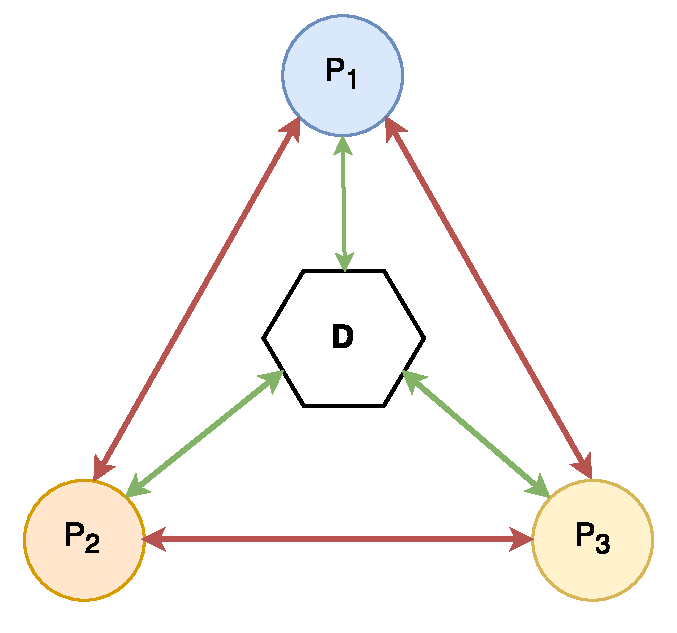
\includegraphics[width=0.5\textwidth]{imagenes/architecture.pdf}
  \caption{Conexión entre nodos \texttt{Directorio} y Participantes}
  \label{fig:connections-directory-participants}
\end{figure}

La funcionalidad de proveer un punto de entrada a la sala también se podría 
realizar entre los propios nodos \texttt{Participantes}, sin la necesidad de 
incorporar un nodo \texttt{Directorio}. Si bien en esta investigación se 
priorizó la facilidad de implementar la variante utilizando el nodo adicional, 
se podría ejecutar alguna variante de \emph{gossip protocol} 
\cite{Demers:1987:EAR:41840.41841} para informar la identidad de participantes 
nuevos que vayan entrando a la sala, lo cual podría solucionar el problema. 
Esta segunda variante además tiene la ventaja de no poseer un punto vulnerable 
(que sería el nodo \texttt{Directorio}), evitando ataques directos al nodo 
\texttt{Directorio}, retrasando (o incluso imposibilitando) la 
creación del \emph{anonymity set}. 

Actualmente el nodo \texttt{Directorio} inicia estableciendo los 
parámetros públicos del protocolo y publica su dirección IP. Luego, cada nodo 
Participante que se quiera unir se conecta a la dirección pública del 
\texttt{Directorio} y espera que se complete la cuota de participantes 
establecida en un comienzo. Cuando se conectan los $n$ participantes 
necesarios, el \texttt{Directorio} informa la dirección IP de cada uno de los 
participantes a todo el resto, para que posteriormente inicien el protocolo 
solo enviándose mensajes entre ellos. Esto termina la labor del nodo 
\texttt{Directorio}. En la Figura \ref{fig:connections-directory-participants} 
se observa las conexiones que se realizan durante el desarrollo del protocolo, 
primero conectando cada participante que viene entrando a la sala al nodo 
\texttt{Directorio} (representado por las conexiones verdes), y luego que 
todos los participantes se hayan conectado al nodo \texttt{Directorio}, éste 
le comunica a toda la sala las direcciones de los nodos \texttt{Participantes} 
presentes, terminando su labor, desconectándose de los nodos 
\texttt{Participantes}, y estos finalmente se conectan mediante los enlaces 
rojos entre cada uno de ellos. En la Figura \ref{fig:connections-participants} 
se observa en mayor detalle la conexión entre cada par de participantes, la 
cual se realiza a través de \emph{sockets} tipo \emph{requestor-replier}, 
formando así el \emph{anonymity set} deseado, y continuando con el normal 
desarrollo del protocolo anteriormente descrito.

\begin{figure}[H]
  \centering
    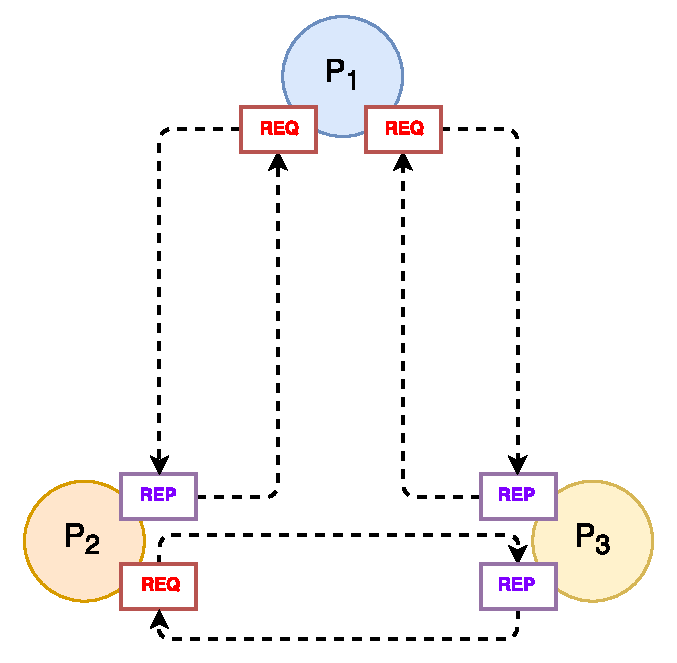
\includegraphics[width=0.5\textwidth]{imagenes/participants_connection.pdf}
  \caption{Conexión entre nodos \texttt{Participantes}}
  \label{fig:connections-participants}
\end{figure}

\section{Primitivas Criptográficas}

En la implementación actual, la gran mayoría de las primitivas criptográficas 
han sido implementadas desde cero, valiéndose principalmente de la biblioteca 
para manejar números grandes de \emph{Java}, \emph{BigInteger}\footnote{\url{
https://docs.oracle.com/javase/7/docs/api/java/math/BigInteger.html}}. Si bien 
esto no es una práctica recomendada (lo ideal es utilizar bibliotecas 
criptográficas ya probadas por la comunidad), se decidió por esto luego de no 
encontrar bibliotecas que implementaran las funcionalidades requeridas por el 
protocolo (\emph{Pedersen Commitments} y \emph{ZKP} asociadas). Como fue 
dicho, la implementación de primitivas criptográficas no es recomendado, más 
bien, se recomienda utilizar implementaciones ya probadas y verificadas por la 
comunidad, como lo podría ser 
Charm-Crypto\footnote{\url{http://charm-crypto.com/index.html}} o 
Scapi\footnote{\url{https://scapi.readthedocs.io/en/latest/}}. De todas 
maneras, la criptografía implementada se desarrolló utilizando interfaces, por 
lo que de tener una librería que cumpla los requerimientos criptográficos 
indicados en el Capítulo 3, su implantación podrá ser realizada de manera 
expedita y transparente al resto de la implementación.

\section{\emph{API} implementada}

Como fue dicho anteriormente, una contribución importante de este trabajo 
es implementar una \emph{API} disponible para toda la comunidad. Esta API 
permitirá a la comunidad crear una aplicación que esté basada en el protocolo 
anteriormente descrito. 

La implementación anterior fue empaquetada como librería \emph{Java}, 
utilizable por otras aplicaciones al importar el archivo \emph{.jar} generado. 
Esta librería quedó con los siguientes métodos de manera pública, formando así 
la \emph{API} disponible:

\begin{itemize}
    \item \texttt{DCNETProtocol class:} clase base que entrega la \emph{API} 
    que es necesario instanciar para utilizar los métodos descritos a 
    continuación. 
    \item \texttt{boolean connectToDirectory():} luego de setear la dirección 
    IP del nodo \texttt{Directorio}, este método realiza la conexión desde el 
    nodo \texttt{Participante} hacia el \texttt{Directorio}, utilizando las 
    funciones provistas por la librería \emph{ZeroMQ}.
    \item \texttt{void setMessageToSend(String s, boolean b):} este método 
    tiene como finalidad permitir al nodo \texttt{Participante} establecer el 
    mensaje que desea comunicar al resto de la sala utilizando el protocolo. 
    \item \texttt{void runProtocol(PrintStream p):} corre el protocolo 
    anteriormente descrito de manera automática, calculando los diferentes 
    \emph{commitments} y \emph{zero-knowledge proofs} necesarios, repitiendo 
    las rondas necesarias y finalizando cuando todos los mensajes han sido 
    recibidos por la totalidad de los participantes en cuestión.
    \item \texttt{ObservableParticipantsLeft:} objeto que emplea el patrón de 
    diseño \emph{Observer} para ir informando cuáles participantes se van 
    conectando a la sala a medida que va ocurriendo, y así tener una noción de 
    cuantos participantes faltan para completar la cuota puesta en un 
    principio por el nodo \texttt{Directorio}.
    \item \texttt{ObservableMessagesArrived:} también emplea el patrón de 
    diseño \emph{Observer} para informar al participante de los mensajes que 
    van resultando de correr el protocolo, a medida que éste avanza. 
    Importante señalar que los mensajes se despliegan en tiempo real.
\end{itemize}

\section{Aplicación Móvil}

Para poder probar el uso de la \emph{API} implementada, se desarrolló una 
aplicación móvil prototipo, que tiene como objetivo permitir un uso 
simplificado 
del protocolo implementado, que permita a los usuarios montar una conversación 
que asegure el anonimato de sus participantes.

La aplicación está compuesta de 3 módulos: (1) conexión al nodo 
\texttt{Directorio}, (2) envío del mensaje por parte del participante, y (3) 
recepción de los mensajes del resto de los participantes de la sala.

\begin{figure}[H]
    \centering
    \begin{subfigure}[b]{0.4\textwidth}
        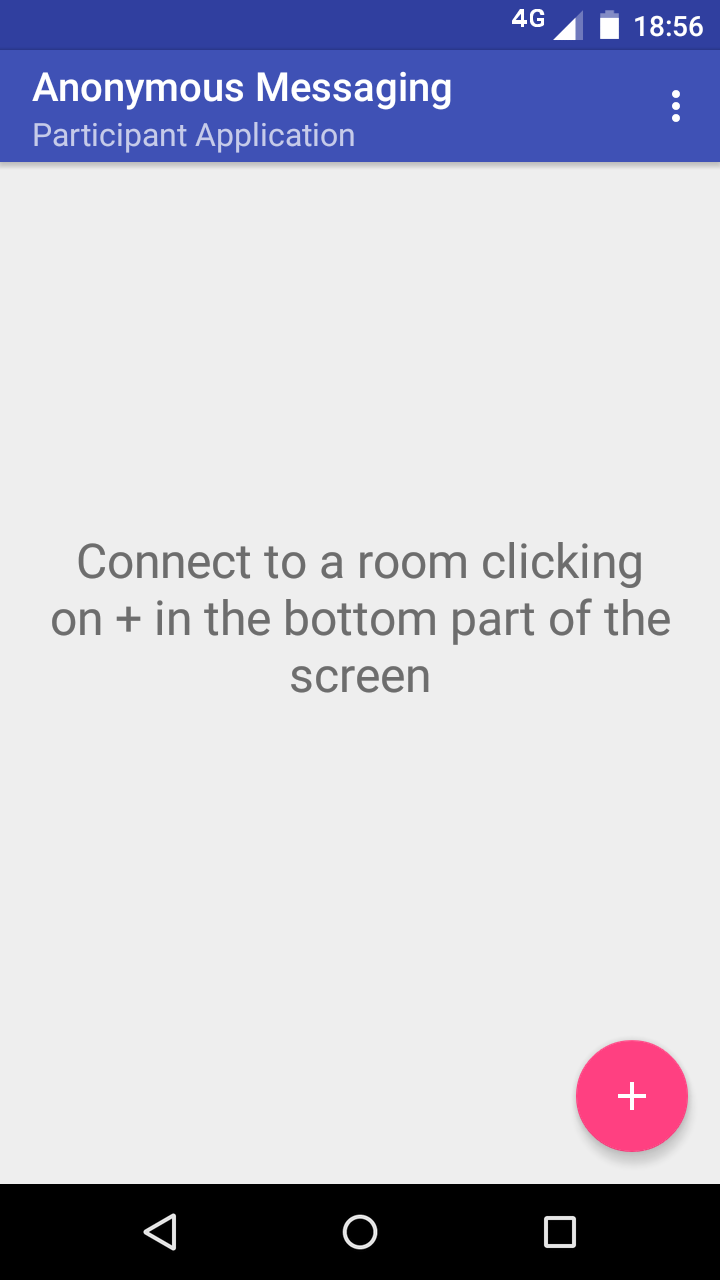
\includegraphics[width=\textwidth]{imagenes/mobile_first.png}
        \caption{Conexión al Nodo \texttt{Directorio}}
        \label{fig:mobile_connect}
    \end{subfigure}
    ~
    \begin{subfigure}[b]{0.4\textwidth}
        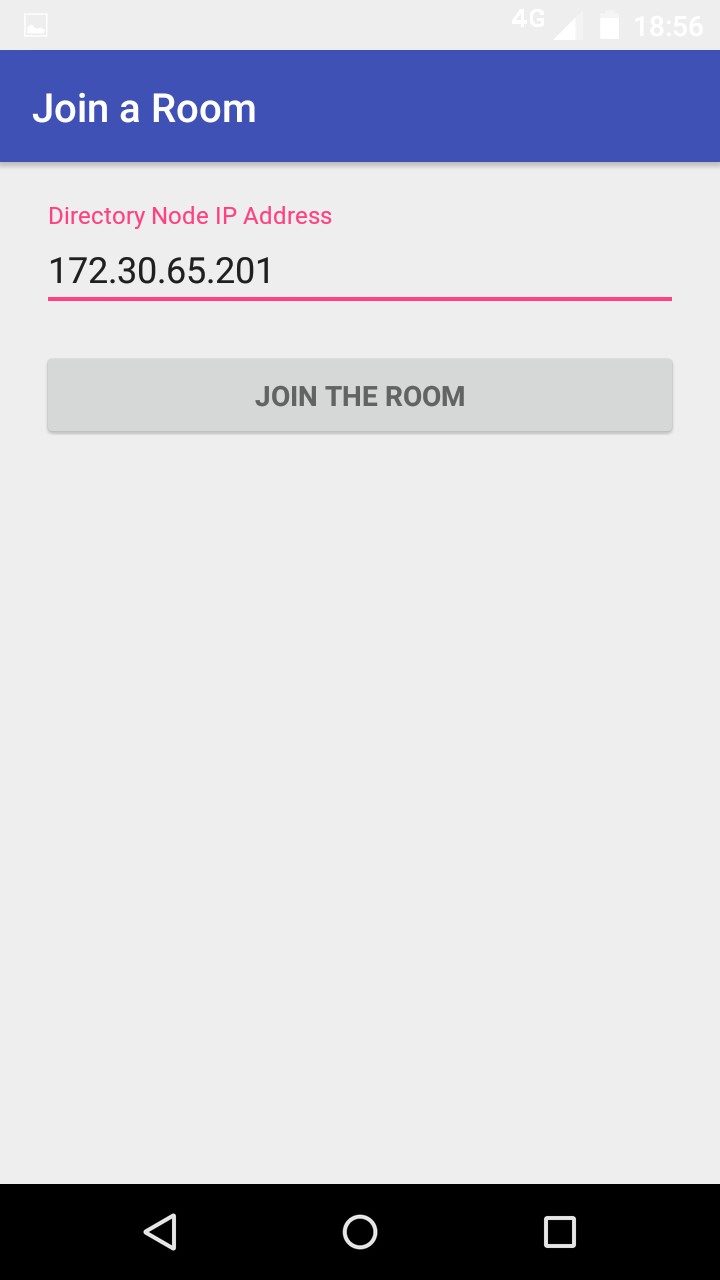
\includegraphics[width=\textwidth]{imagenes/mobile_connect.png}
        \caption{Establecer dirección del \texttt{Directorio}}
        \label{fig:mobile_set_ip}
    \end{subfigure}
    \caption{Screenshots de Aplicación Móvil (parte 1)}
    \label{fig:mobile_screenshots_1}
\end{figure}

\begin{figure}[H]
    \centering
    \begin{subfigure}[b]{0.4\textwidth}
        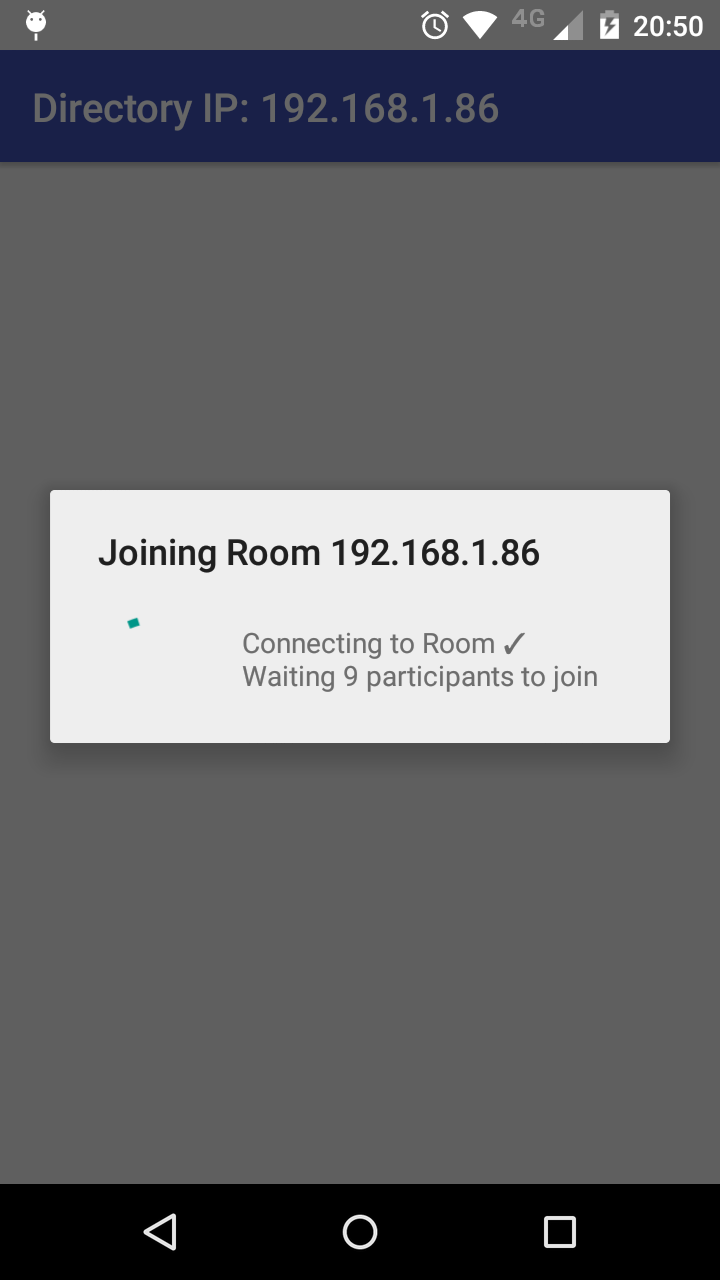
\includegraphics[width=\textwidth]{imagenes/mobile_connecting.png}
        \caption{Esperando conexión a Sala}
        \label{fig:mobile_waiting}
    \end{subfigure}
    ~
    \begin{subfigure}[b]{0.4\textwidth}
        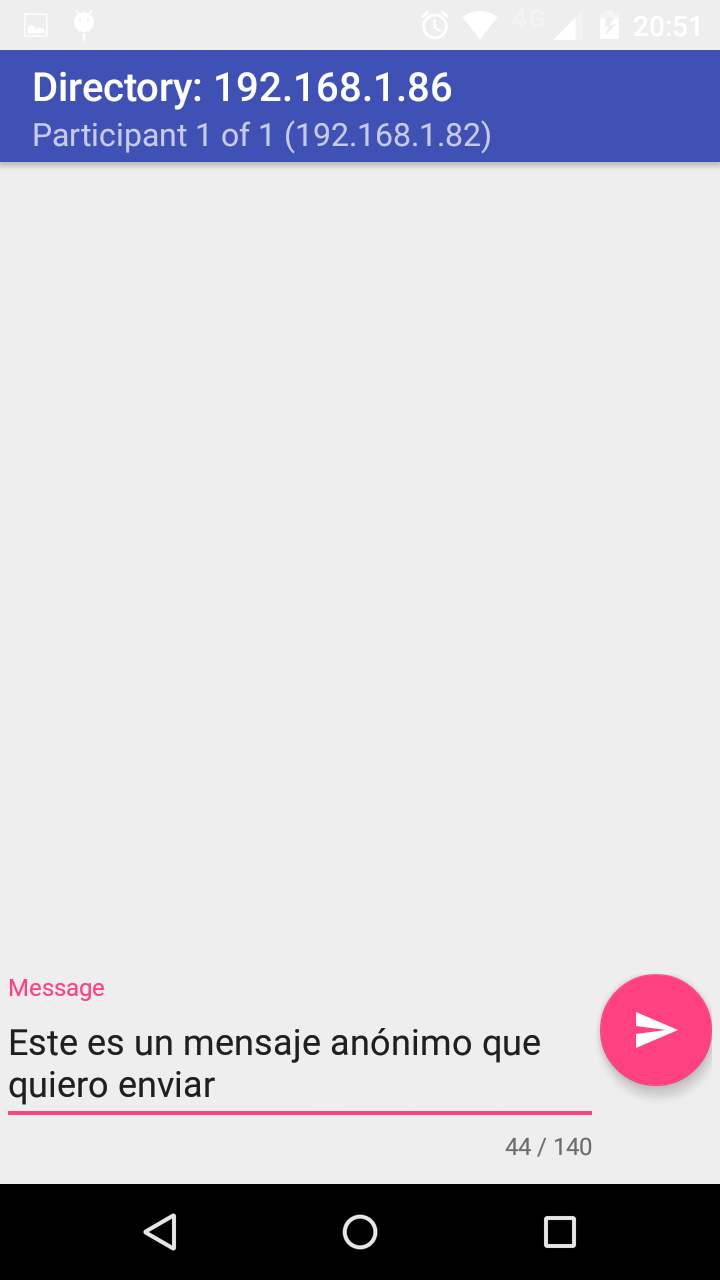
\includegraphics[width=\textwidth]{imagenes/mobile_message.png}
        \caption{Envío del mensaje a la sala}
        \label{fig:mobile_set_msg}
    \end{subfigure}
    \caption{Screenshots de Aplicación Móvil (parte 2)}
    \label{fig:mobile_screenshots_2}
\end{figure}
